\svnidlong
{$LastChangedBy$}
{$LastChangedRevision$}
{$LastChangedDate$}
{$HeadURL$}

\chapter{Particle tracking}
\label{ch:tracking}

In this chapter, we will explain the method used to extract the three dimensional coordinates and trajectories of colloidal particles from the confocal microscope images. This analysis is the basis of the rest of the work in this thesis.

\section{Principle}
More than a century ago, Jean Perrin~\citep{perrin} was measuring coordinates of thousands of Brownian particles on photographic plate with a ruler to prove the sedimentation-diffusion equilibrium. Nowadays, we can program computers to perform the same tedious task. Modern particle tracking by computer image analysis was pioneered by John C. Crocker and David C. Grier~\citep{crocker1996mdv}. Originally a two dimensional process, the algorithm was extended in two ways to treat confocal three-dimensional images. The first method consist in dealing directly with 3D images: each step of the algorithm is implemented in three dimensions~\citep{dinsmore2001tdc}. The second method is to track particles in each 2D slice and then reconstruct a set of coordinate in 3D by another method~\citep{vanblaaderen1995rss, Lu2007, Lu2008}.

In this section, we will describe how does the \ac{CG} algorithm works. In the next section we will detail why and how we re-implemented this algorithm to fit our needs.

\begin{figure}
	\centering
	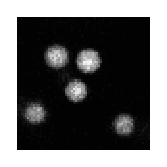
\includegraphics[width=0.3\textwidth]{dillute_raw}
	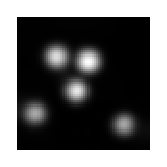
\includegraphics[width=0.3\textwidth]{dillute_filtered}
	
\includegraphics[width=0.3\textwidth]{dillute_centers}\\
	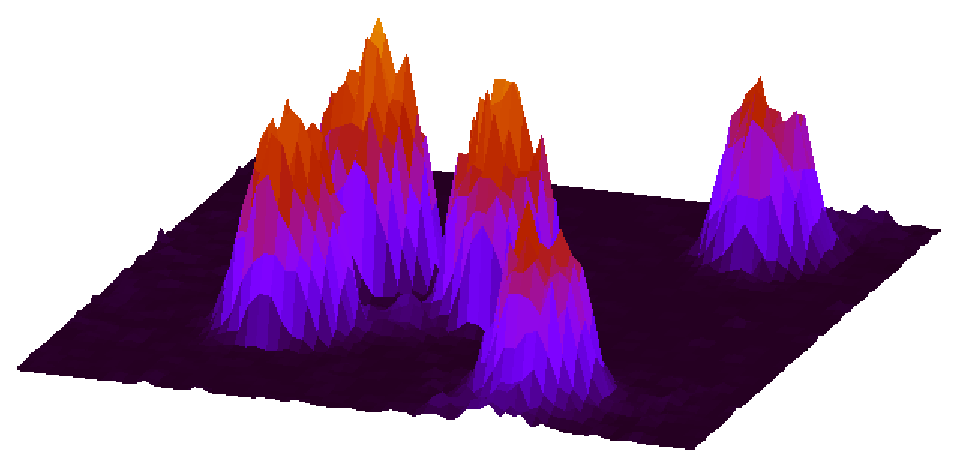
\includegraphics[width=0.3\textwidth]{dillute_raw_gp_raster}
	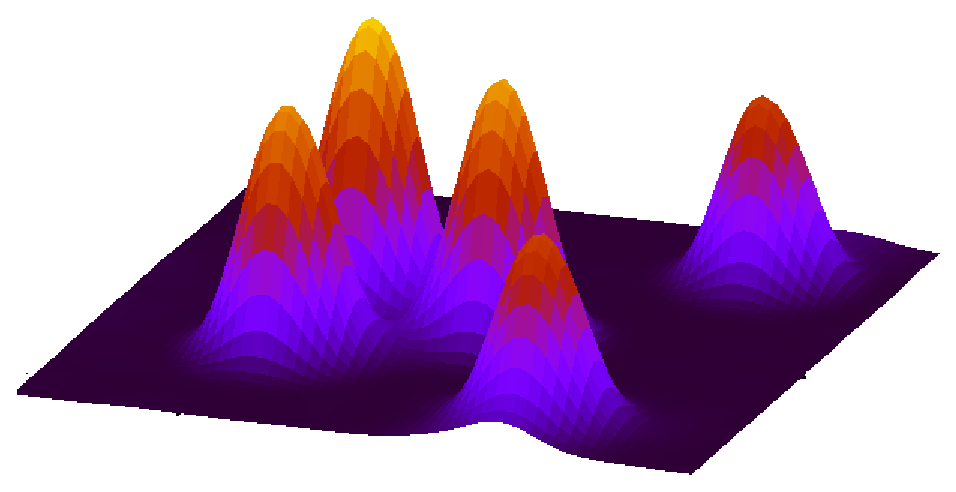
\includegraphics[width=0.3\textwidth]{dillute_filtered_gp_raster}
	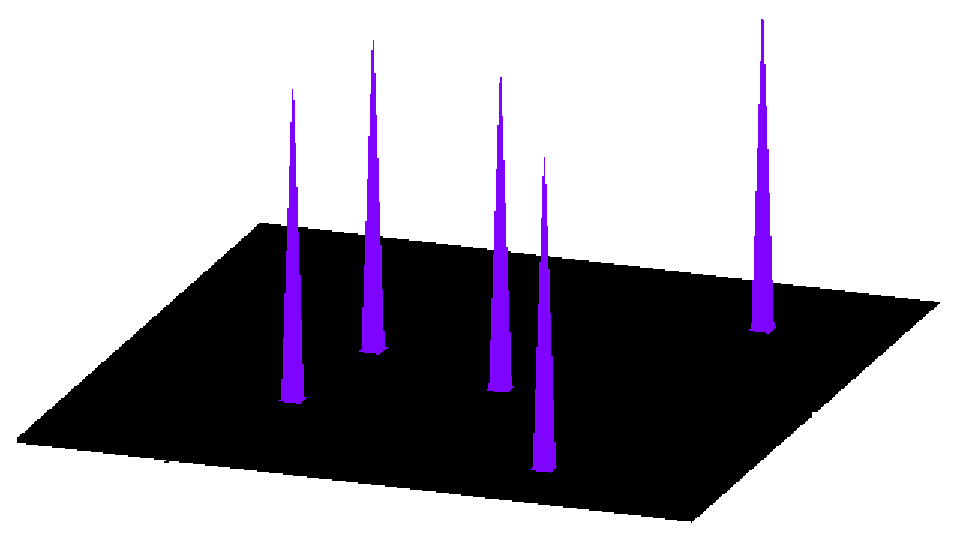
\includegraphics[width=0.3\textwidth]{dillute_centers_gp_raster}
\caption{Schematic Crocker and Grier algorithm in 2D for a dilute sample. The bottom part represent the same image as the top, but with an elevation corresponding to the pixel intensity. Left: Original image. The image noise, at a length scale of a few pixels is particulary apparent in the bottom representation. Middle: Filtered image. The noise has been reduced so that each particle appears as a smooth blob. Right: Tracked centres (low intensity centres were removed).}
\label{fig:track2D}
\end{figure}

The process of the \ac{CG} algorithm is sketched in \FigureRef{fig:track2D} for a 2D image in a simple dilute case. Tracking is done in three steps in each picture (2D or 3D).
\begin{enumerate}
	\item The images are filtered in order to have a Gaussian-like bright blob on a dark background for each particle. 
	\item Potential centres are identified as the pixels that are local intensity maxima (top of the blobs). Most of the time a threshold is needed to discard local maxima due to noise in the (almost) black background.
	\item The precision is refined to sub-pixel by taking the centroid (centre of mass) of the neighbouring pixels.
\end{enumerate}

And finally, the coordinates are linked from time step to time step into trajectories. This last step is not a graphical operation and thus is not included in the tracker. It will be discussed in \SectionRef{sec:time_tracking}.

The \ac{CG} algorithm can seem rough, almost too simple. However it works well with almost identical isotropic objects like spheres. It is known~\citep{crocker1996mdv} to achieve routinely a precision of a tenth of a pixel ($\sim\sigma/100$) in a 2D picture containing hundreds of particles. At the same time, this algorithm has a small set of parameters which allows adaptation to various image quality and experimental conditions. It's main limitation is the polydispersity of the particles. If the particles have too disparate sizes, a multiscale approach~\citep{Adelson1984, Lindeberg1993, OlivoMarin2002, Hinz2005} becomes necessary, but this goes beyond the scope of this thesis. 



\subsection{Image filtering}

\begin{figure}
	\centering
	\subfloat[Not enough blurring]{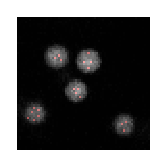
\includegraphics[width=0.4\textwidth]{dillute_notblured}}\quad
	\subfloat[Too much blurring]{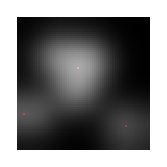
\includegraphics[width=0.4\textwidth]{dillute_tooblured}}
	\caption{The same image as in \FigureRef{fig:track2D} with different amount of blurring. Tracked centres are displayed in red.}
	\label{fig:bad_blur}
\end{figure}

Confocal imaging is a trade-off between reducing the thickness of the focal plane and allowing enough light to go through the pinhole. Other constrains, like the need form rapid data acquisition, contribute to make an actual confocal image often noisier than a usual optical microscope image. The noise exists typically on a length scale of a few pixels. Cutting the high frequencies of the image, or equivalently convolving the image with a Gaussian kernel, will remove the noise. The particles will then appear as smooth blobs. The cut-off frequency, or the size of the Gaussian kernel, is crucial (see \FigureRef{fig:bad_blur}). A little bit too much blurring would smear out the smaller particles. Even more blurring and the blobs of the particles begin to merge, leading to ill defined coordinates. Leaving too many high frequencies is not good either, because it allows multiple local maxima per particle, leading to inconsistent tracking.

\begin{figure}
	\centering
	\def\svgwidth{\textwidth}
	\input{track1D.pdf_tex}
	\caption{Schematic 1D picture of the possible distortions of the input image. Top-right: A perfect signal that may correspond to a 1D crystal of slightly polydisperse particles. Each intensity plateau is a particle. Bottom-right: Same signal, but with large scale intensity variation and a small amount of noise. Bottom-left: Same as previous, but with a larger amount of noise. Top-left: Same signals as bottom-left (red) and bottom-right (green) after band-pass filtering. The straight (blue) line is the zero after filtering. Peaks will be detected as particle centres.}
	\label{fig:track1D}
\end{figure}

Image overall intensity can vary quite a lot in space. This can be due to light absorption by the sample, large scale optical aberration and bleaching of the fluorescence. Because the sample absorbs light, the top of the image stack (closer to the objective lens) will be brighter than the bottom (further from the objective lens). One can compensate for this effect at acquisition time by making the gain and the offset of the \ac{CCD} camera $Z$-dependant. At low zoom, one can observe that the centr of a given $XY$ image is brighter than the edges. This effect can be particularly strong in the corners. Furthermore, after some time under the laser, the fluorescent dye beaches. This makes the colloids dimmer. But the colloids that are outside the scanned area do not receive laser light and so stay bright. A problem arises when such unbleached particles diffuse inside the scanned area. Thus, with time, the centre of the scanned area becomes dimmer and dimmer, whereas the edges are populated partly by bright particles from the outside. Both optical aberrations and bleaching cannot be compensated at acquisition time, so a 3D picture out of the scanning confocal microscope is typically heterogeneous in intensity.

Another cause of heterogeneous intensity is intrinsic to the colloids. During the synthesis, a small fraction of the colloids are labelled with much less dye than average; then looking dim under fluorescent microscopy. Conversely, a small fraction of the colloids appear very bright. The later is not a problem, even if the image saturates, but the dim particles are erroneously removed by a threshold that usually distinguish well between particles and noise.

For any of these reasons, it is often useful to remove the low frequencies of the image, except maybe at low density when the background is almost perfectly dark. At low and moderate densities, a high-pass filter has to be tuned carefully if used. If we cut intensity variations at length scales smaller than the distance between two particles, a bright artefact may appear between them. Cut-off length scales of the order of the particle diameter can only be applied at very high densities, were there is no void larger than the particle size. This is only in this latter case that we are able to track a very dim particle surrounded by much brighter particles.

In any case, if the image is band-passed, the two cutting length scales (or frequencies) must be separated by at least a factor 2. If not, the filter will select only a narrow band of frequencies, enhancing random features of the image or even the edges of the particles instead of their centres.

Band pass filtering is often implemented in that way: two copies of the original image are made and blurred by a Gaussian filters of different size. The small-blurred one has the noise removed but brightness heterogeneities remain. The large-blurred one has all the features of the size of the particles erased, keeping only the large scale background intensity variations. The subtraction of the two copies yields the band passed image.

\subsection{Selecting local maxima}

After a good filtering, the selected features of the image (hopefully the particles) are bright and smooth Gaussian blobs on a dark background. Thus there should be one and only one local maxima per particle, on top of the blob. Local maxima are often detected using a dilation filter. Dilation is a morphological filter that assigns to each pixel the maximum brightness of its neighbourhood. This filter was easy to use because it is implemented in in most of the image processing software and libraries (Photoshop, IDL, Intel primitives, etc.). A copy of the filtered image is dilated and compared to the original (filtered) copy. The pixels that have the same value in both versions are the local maxima.

Some local maxima may exist outside any particle. They may be due to noise or to the light coming from an out-of-plane particle because our microscope is diffraction limited (this last effect is drastically reduced if the filtering was done in 3D). Usually, these local maxima have much lower intensities than those corresponding to a particle. They can be easily discarded by a threshold in brightness.

Bad low frequency filtering usually causes many false positive detections. It enhanced dim features far from any particle. It is then impossible to tell them apart by the intensity threshold.

In dense samples, there is no void large enough to host a local maximum. Thresholding is then unnecessary, or even counter-productive because one may discard dim particles.

\subsection{Sub-pixel resolution}

After the detection of local maxima and thresholding, we are be able to assign a pixel to each particle. Our precision is the size of a pixel, typically a tenth of the particle diameter. To go beyond, one can fit a Gaussian on the blob around the local maxima. Equivalently, one can calculate the intensity centroid (centre of mass) of the neighbourhood of the local maxima. This refines precision to a tenth of a pixel, \latin{i.e.} $\sim\sigma/100$.

The pitfall here is to take a too large neighbourhood. If two particles are at contact, optical effects, further enhanced by filtering, will skew the two blobs one towards the other~\citep{Baumgartland2005}. If the neighbourhood used for sub-pixel resolution is too wide, one may catch the influence of neighbouring blobs, thus shifting the coordinates of the particles. This effect is notably strong at the interface between a condensed phase and a gas, for example in the case of colloidal gel. Particles at the interface have neighbours only on one side and their tracked coordinates could then be shifted toward the dense phase.

\section{Implementation}

\subsection{Existing implementations}

The \ac{CG} algorithm was implemented already a few times in various flavours by different people in a few programming languages. Of course, there is the original IDL implementation by John Crocker~\citep{crocker1996mdv}, improved by Eric Weeks. This implementation was cloned in Matlab~\citep{BlairDufesneMatlab, Gao2009} and GDL~\citep{Desmond}. We had also access to the personal C++ implementation of Paddy Royall~\citep{Royall2003}. They all use full 3D localisation method. 

The limiting parameter of full 3D localisation method is the memory of the computer, because the whole 3D image has to be loaded in memory. However in all the existing implementations, the details of the program required at least two high precision copies of the image, \latin{i.e.} two blocks of continuous memory of 8 times the disk space used by the uncompressed image. For example, an uncompressed \unit{8}{\bit} grey scale cubic 3D picture of \unit{256}{pixels} in each direction takes \unit{16}{\mega\byte} on disk. To analyse it with the previous implementation one needs at least two blocks of \unit{128}{\mega\byte}. Such amount of working memory was a challenge a few years ago, but is not a big deal for modern computers. However, simply doubling the size of the image (\unit{512}{pixels} cubic) crosses the limit of \unit{1}{\giga\byte} for each memory block, which is impossible for a MS Windows \unit{32}{\bit} computer.

That is with this limitation in mind that the 2D localisation with 3D reconstruction was implemented first in IDL by van Blaaderen and co-workers~\citep{vanBlaaderen1997} back in 1995 and more recently in C++ by \citet{Lu2007}. 2D tracking is inexpensive in memory and can use the standard filters, algorithms and hardware acceleration of image processing that are almost always implemented in two dimensions. However, the reconstruction step makes assumptions on the intensity profile of a particle in the $Z$ direction. This assumption is fair when the imaging quality is good and the particles monodispersed and of equal brightness. With our slightly polydispersed particles, it was impossible to reach a good precision on the $Z$ coordinate.

All the full 3D implementations are slow, taking typically \unit{10}{\minute} per \unit{256}{pixels} cubic images. They need to perform $O(N^2)$ operations, with $N$ the number of pixels in the image. In addition, interpreted languages like IDL or Matlab are not known for their speed performances.

\subsection{Our implementation}

Because we were planning to investigate heterogeneities of about 10 particle sizes, we wanted to track a large number of particles to reach meaningful statistics. We also wanted a good precision on the position of the particles in three dimensions. And we had a to use colloids with a non-negligible amount of polydispersity. With these constrains, no existing implementation was fitting our needs. Moreover, large data meant slower and slower tracking. So we decided to do our implementation in a compiled language (C++) and to look for both speed and memory optimizations.

Our code is available online~\citep{LeocmachColloids} under the GNU General Public License version 3.0.
\begin{figure}
	\centering
	
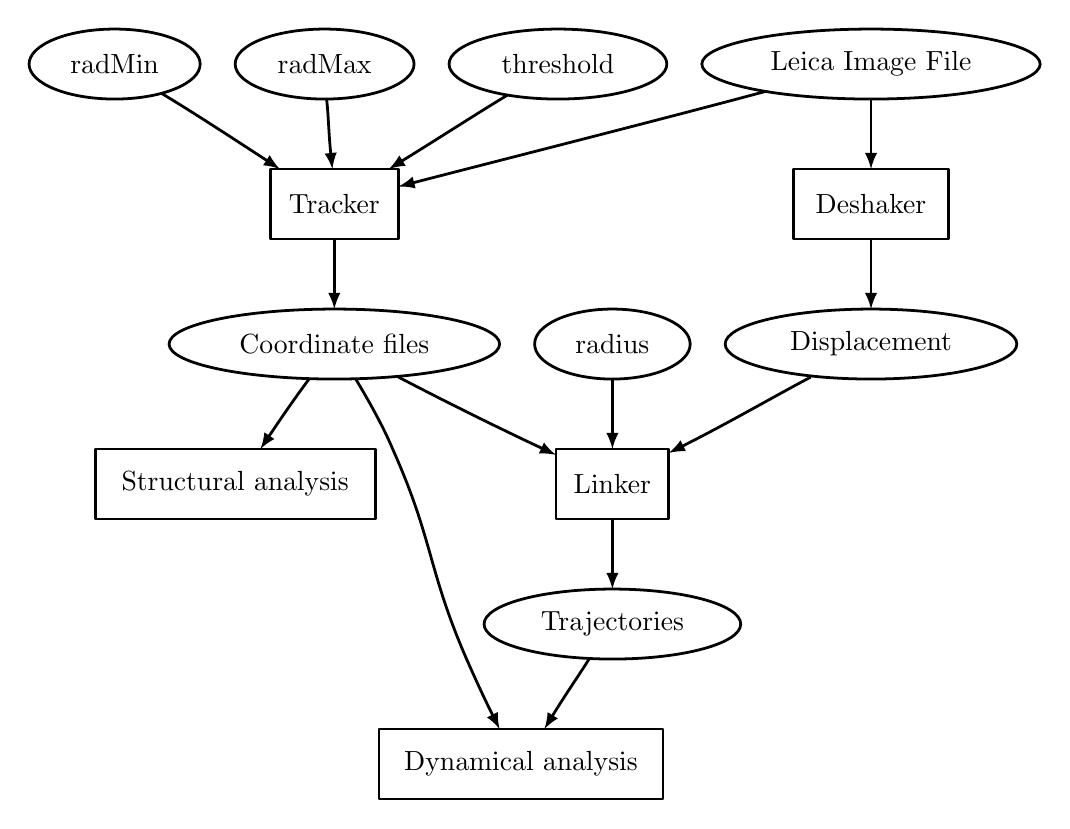
\begin{tikzpicture}[>=latex,line join=bevel,scale=0.7]
  \pgfsetlinewidth{1bp}
%%
\pgfsetcolor{black}
  % Edge: dat_files -> Linker
  \draw [->] (190bp,217bp) .. controls (211bp,206bp) and (239bp,192bp)  .. (271bp,177bp);
  % Edge: threshold -> Tracker
  \draw [->] (246bp,362bp) .. controls (231bp,353bp) and (211bp,340bp)  .. (185bp,324bp);
  % Edge: lif -> Tracker
  \draw [->] (379bp,364bp) .. controls (327bp,350bp) and (248bp,330bp)  .. (190bp,315bp);
  % Edge: dat_files -> Structure
  \draw [->] (144bp,216bp) .. controls (138bp,208bp) and (131bp,198bp)  .. (119bp,180bp);
  % Edge: radMax -> Tracker
  \draw [->] (153bp,360bp) .. controls (154bp,352bp) and (154bp,343bp)  .. (156bp,324bp);
  % Edge: dat_files -> Dynamics
  \draw [->] (168bp,216bp) .. controls (174bp,206bp) and (182bp,192bp)  .. (187bp,180bp) .. controls (208bp,133bp) and (205bp,118bp)  .. (225bp,72bp) .. controls (229bp,63bp) and (233bp,54bp)  .. (242bp,36bp);
  % Edge: lif -> Deshaker
  \draw [->] (433bp,360bp) .. controls (433bp,352bp) and (433bp,343bp)  .. (433bp,324bp);
  % Edge: Tracker -> dat_files
  \draw [->] (157bp,288bp) .. controls (157bp,280bp) and (157bp,271bp)  .. (157bp,252bp);
  % Edge: displ_file -> Linker
  \draw [->] (402bp,217bp) .. controls (383bp,207bp) and (359bp,193bp)  .. (329bp,178bp);
  % Edge: radMin -> Tracker
  \draw [->] (68bp,363bp) .. controls (83bp,354bp) and (103bp,341bp)  .. (129bp,324bp);
  % Edge: radius -> Linker
  \draw [->] (300bp,216bp) .. controls (300bp,208bp) and (300bp,199bp)  .. (300bp,180bp);
  % Edge: Deshaker -> displ_file
  \draw [->] (433bp,288bp) .. controls (433bp,280bp) and (433bp,271bp)  .. (433bp,252bp);
  % Edge: Linker -> traj_file
  \draw [->] (300bp,144bp) .. controls (300bp,136bp) and (300bp,127bp)  .. (300bp,108bp);
  % Edge: traj_file -> Dynamics
  \draw [->] (288bp,72bp) .. controls (283bp,64bp) and (276bp,54bp)  .. (265bp,36bp);
  % Node: radMin
\begin{scope}
  \pgfsetstrokecolor{black}
  \draw (44bp,378bp) ellipse (44bp and 18bp);
  \draw (44bp,378bp) node {radMin};
\end{scope}
  % Node: lif
\begin{scope}
  \pgfsetstrokecolor{black}
  \draw (433bp,378bp) ellipse (87bp and 18bp);
  \draw (433bp,378bp) node {Leica Image File};
\end{scope}
  % Node: displ_file
\begin{scope}
  \pgfsetstrokecolor{black}
  \draw (433bp,234bp) ellipse (75bp and 18bp);
  \draw (433bp,234bp) node {Displacement};
\end{scope}
  % Node: Linker
\begin{scope}
  \pgfsetstrokecolor{black}
  \draw (329bp,180bp) -- (271bp,180bp) -- (271bp,144bp) -- (329bp,144bp) -- cycle;
  \draw (300bp,162bp) node {Linker};
\end{scope}
  % Node: dat_files
\begin{scope}
  \pgfsetstrokecolor{black}
  \draw (157bp,234bp) ellipse (85bp and 18bp);
  \draw (157bp,234bp) node {Coordinate files};
\end{scope}
  % Node: traj_file
\begin{scope}
  \pgfsetstrokecolor{black}
  \draw (300bp,90bp) ellipse (66bp and 18bp);
  \draw (300bp,90bp) node {Trajectories};
\end{scope}
  % Node: Tracker
\begin{scope}
  \pgfsetstrokecolor{black}
  \draw (190bp,324bp) -- (124bp,324bp) -- (124bp,288bp) -- (190bp,288bp) -- cycle;
  \draw (157bp,306bp) node {Tracker};
\end{scope}
  % Node: radius
\begin{scope}
  \pgfsetstrokecolor{black}
  \draw (300bp,234bp) ellipse (40bp and 18bp);
  \draw (300bp,234bp) node {radius};
\end{scope}
  % Node: threshold
\begin{scope}
  \pgfsetstrokecolor{black}
  \draw (272bp,378bp) ellipse (56bp and 18bp);
  \draw (272bp,378bp) node {threshold};
\end{scope}
  % Node: Dynamics
\begin{scope}
  \pgfsetstrokecolor{black}
  \draw (326bp,36bp) -- (180bp,36bp) -- (180bp,0bp) -- (326bp,0bp) -- cycle;
  \draw (253bp,18bp) node {Dynamical analysis};
\end{scope}
  % Node: Deshaker
\begin{scope}
  \pgfsetstrokecolor{black}
  \draw (473bp,324bp) -- (393bp,324bp) -- (393bp,288bp) -- (473bp,288bp) -- cycle;
  \draw (433bp,306bp) node {Deshaker};
\end{scope}
  % Node: Structure
\begin{scope}
  \pgfsetstrokecolor{black}
  \draw (178bp,180bp) -- (34bp,180bp) -- (34bp,144bp) -- (178bp,144bp) -- cycle;
  \draw (106bp,162bp) node {Structural analysis};
\end{scope}
  % Node: radMax
\begin{scope}
  \pgfsetstrokecolor{black}
  \draw (152bp,378bp) ellipse (46bp and 18bp);
  \draw (152bp,378bp) node {radMax};
\end{scope}
%
\end{tikzpicture}


	\caption{End user view of the tracking process.}
	\label{fig:tracking_process}
\end{figure}


\subsubsection{Filtering}

The main innovation is that the image filtering is done in Fourier space. The original image is first Fourier transformed, then multiplied by a band-pass mask and finally inverse transformed. The advantage of this method are both in terms of memory and of speed. For the Fourier transforms, we used the very fast FFTW library~\citep{Frigo2005} that allows
\begin{itemize}
	\item At most $O(N\log N)$ operations, with $N$ the number of pixels. 
	\item In-place real discrete Fourier transforms: only one memory block is needed instead of two. 
	\item Single-precision floating point numbers, sufficient for our purpose and consuming half the memory imprint of the double-precision floating point numbers handled by IDL. The memory block is then only 4 times the size of the uncompressed 3D image.
\end{itemize}

The filter is a 3D binary (boolean pixels, \unit{1}{\bit}) image taking a negligible amount of space in memory. A band pass filter is simply a spherical shell that can be drawn once and then applied on every 3D spectrum of a time series. The multiplication take a negligible number of operations ($O(N)$).

\subsubsection{Local maxima}

A second innovation is to compute the local maxima locally, without dilation filter, thus with only one copy of the image. In addition, the order of local maxima finding and thresholding is reversed: The pixels with an intensity below the threshold are not investigated as potential local maxima. In dilute sample, this little trick can speed up the local maxima detection by a factor 20.

\subsubsection{Conclusion}

At the end of the day, the memory imprint of a \unit{256}{pixels} cubic image is reduced to a block of \unit{64}{\mega\byte} that contains the image or the spectrum and a block of \unit{2}{\mega\byte} for the mask. Tracking is done in less than a second on a Intel i7 computer. A image of \unit{512}{pixels} cubic has a total imprint of \unit{528}{\mega\byte} and is tracked in \unit{4}{\second}. With such performance we were able to cope with the GigaBytes of data needed to study supercooled liquids. In the future, we hope this will allows us to look for rare events, like homogeneous crystal nucleation.

\section{Choosing tracking parameters}

\subsection{The parameters}

\ac{CG} algorithm offers three parameters one can tune to get the best tracking of a given dataset. In our implementation, they are to be set in the following order.
\begin{description}
	\item[$r_{min}$] \hfill \\
		The blurring radius, \latin{i.e.} the inverse of the cut-of frequency of the low-pass filter, \latin{i.e.} the maximum length scale of the noise.
	\item[$r_{max}$] \hfill \\
		The inverse of the cut-of frequency of the high-pass filter, \latin{i.e.} the minimum length scale of background intensity variations. The high-pass filter can be totally disabled.
	\item[threshold] \hfill \\
		The minimum intensity that a local maxima must have to be considered a particle centre.
\end{description}

\subsection{General method}

Usually our goal is to track all the particles, whatever their size, and to minimize the tracking errors.

First, try to track a stack for various values of $r_{min}$ without high-pass filter and with a threshold at one quarter of the intensity scale of the image (if the pixel intensity goes from 0 to 255, choose a threshold of 64). The number $N$ of tracked particles function of the blurring radius $r_{min}$ should decrease steeply and then plateau with a slight decreasing slope. The good $r_{min}$ should be set at the very beginning of the plateau. It corresponds to the degree of blurring where the roughness of the intensity profile of the particles has disappeared, but the smaller particles have not yet been smeared out. For us, this value was typically around 3.

Second, have a try with the last stack of the time series. It is the most bleached 3D image, so the dimmer and the one with the poorest signal to noise ratio. If the sample is dense, try with zero threshold and check that no unwanted centre had appeared. If so, the threshold can be kept at zero. If not, it means that the sample is too dilute. Raise progressively the threshold until no noise is caught in the dark background.

Third, if large brightness inhomogeneities are present in the image that prevents to set an uniform threshold, try to use lower and lower values of $r_{max}$, starting at half the size of the image and dividing by 2 at each step. If the goal is only to correct large scales inhomogeneities, especially if the sample is dilute, don't go too low in $r_{max}$ or artefacts will appear in the voids. 

Fourth, if the sample is very concentrated, without voids and if dim particles are present, $r_{max}$ can be set even lower. Be careful though to always keep $2r_{min} \leq r_{max}$.

This is of course not a definitive user manual but only guidelines valid in the few types of samples we were able to test our tracking program on. There is no better tracker than the human eye, so double-check the tracked coordinates against the original images. For dilute samples, a 3D check like in \FigureRef{fig:compare_image_tracked3D} is efficient. For dense samples a check on a random 2D slice is better.

\begin{figure}
	\centering
	\subfloat
		[3D representation of a confocal image (no filtering). Dark pixels are transparent, bright pixels are opaque with a colour going from blue to red with the intensity.]
		{\label{fig:compare_image_tracked3D_image}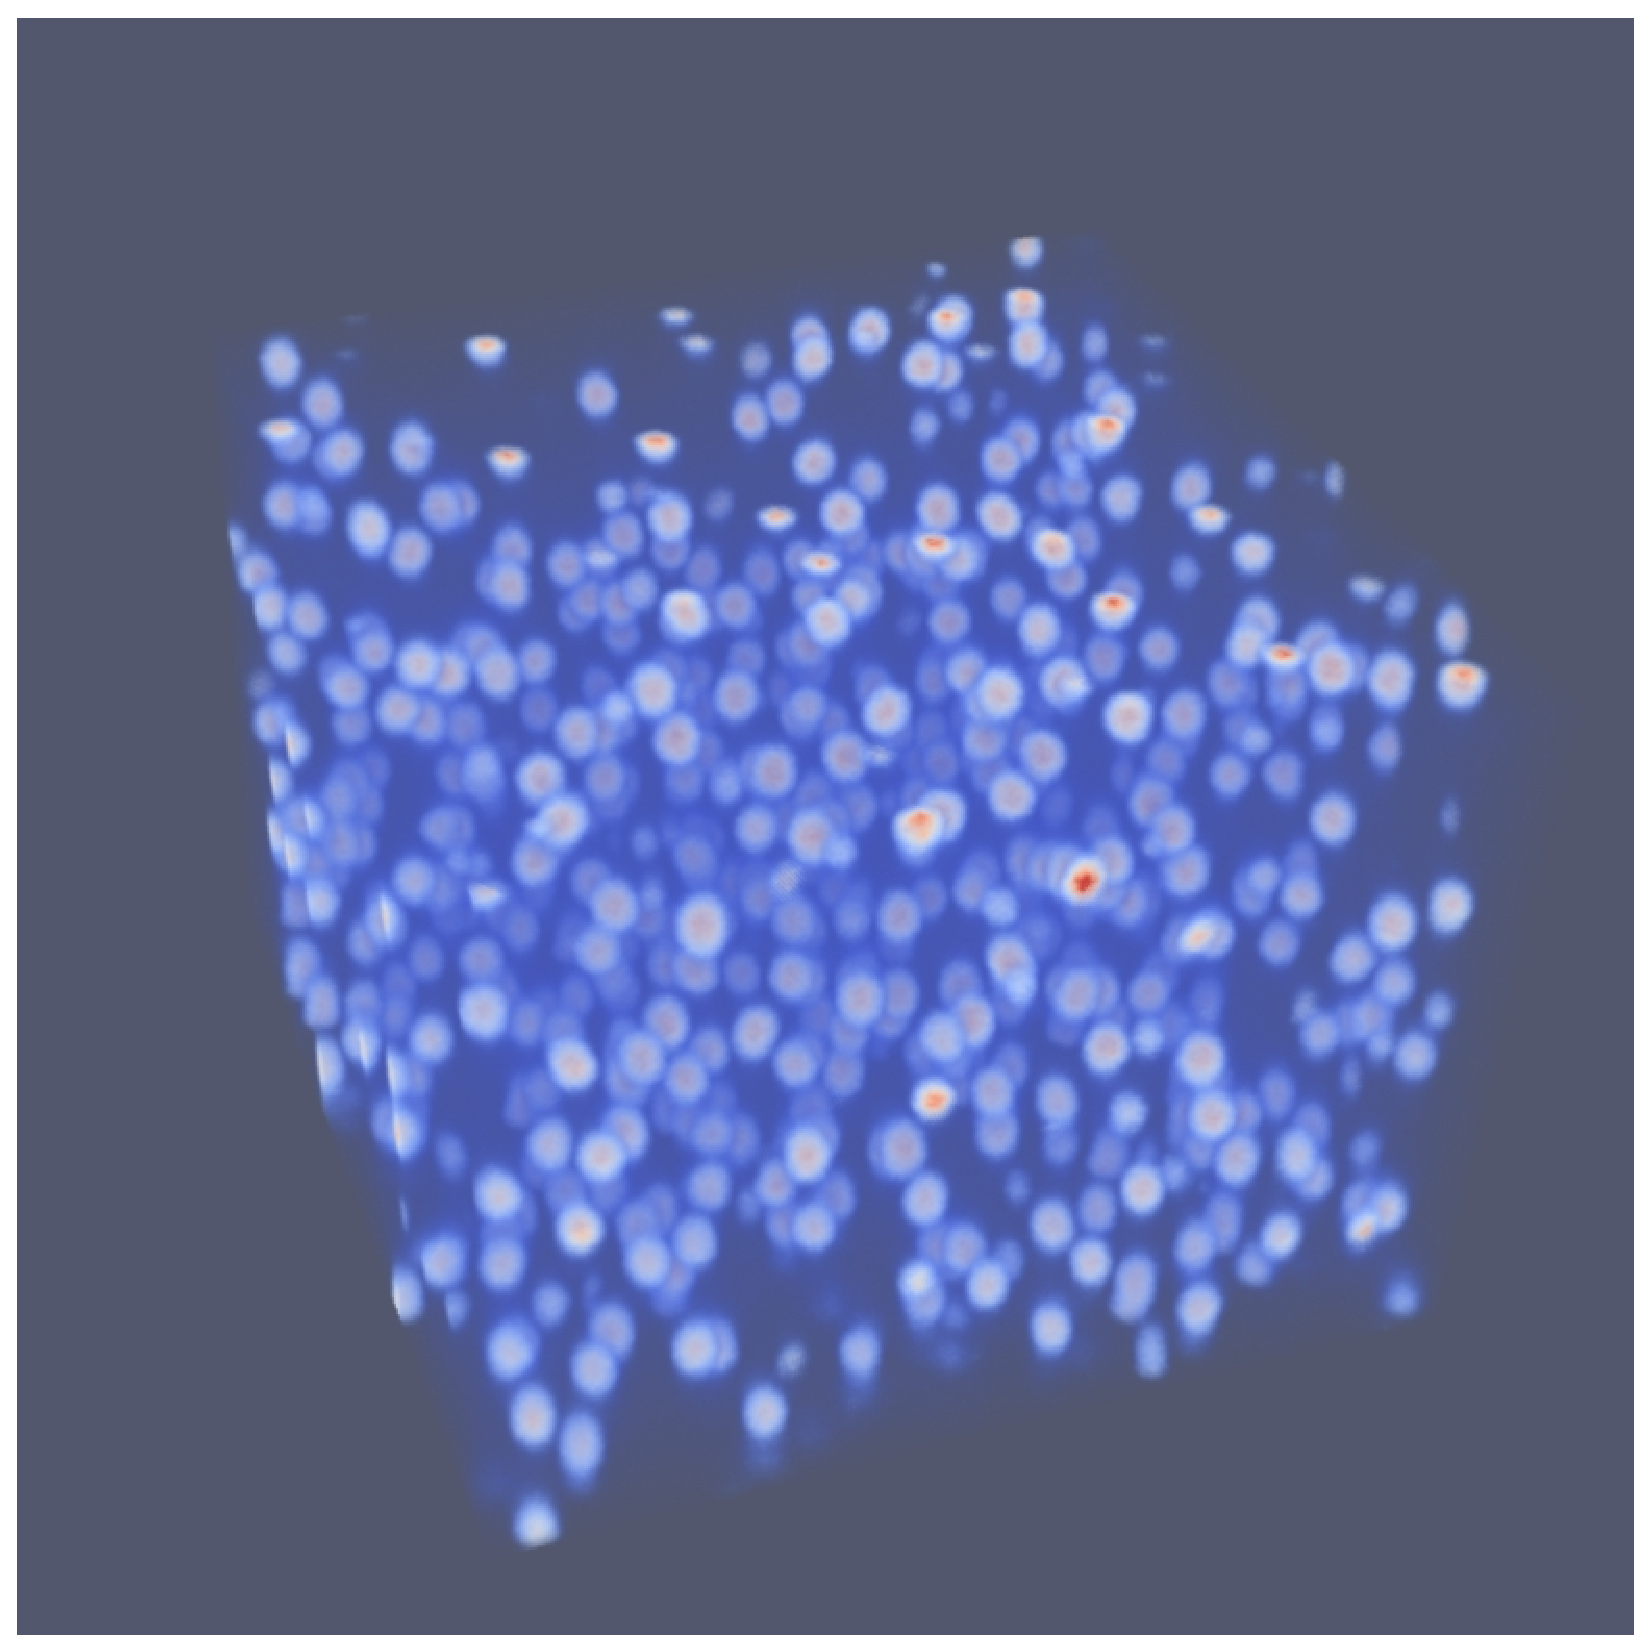
\includegraphics[width=0.45\textwidth]{compare_image_tracked3D_0}}\quad
	\subfloat
		[Plot of the tracked centres. Each sphere has the same diameter (\unit{10}{pixels}). The frame represents the boundary of the picture of the left.]
		{\label{fig:compare_image_tracked3D_plot}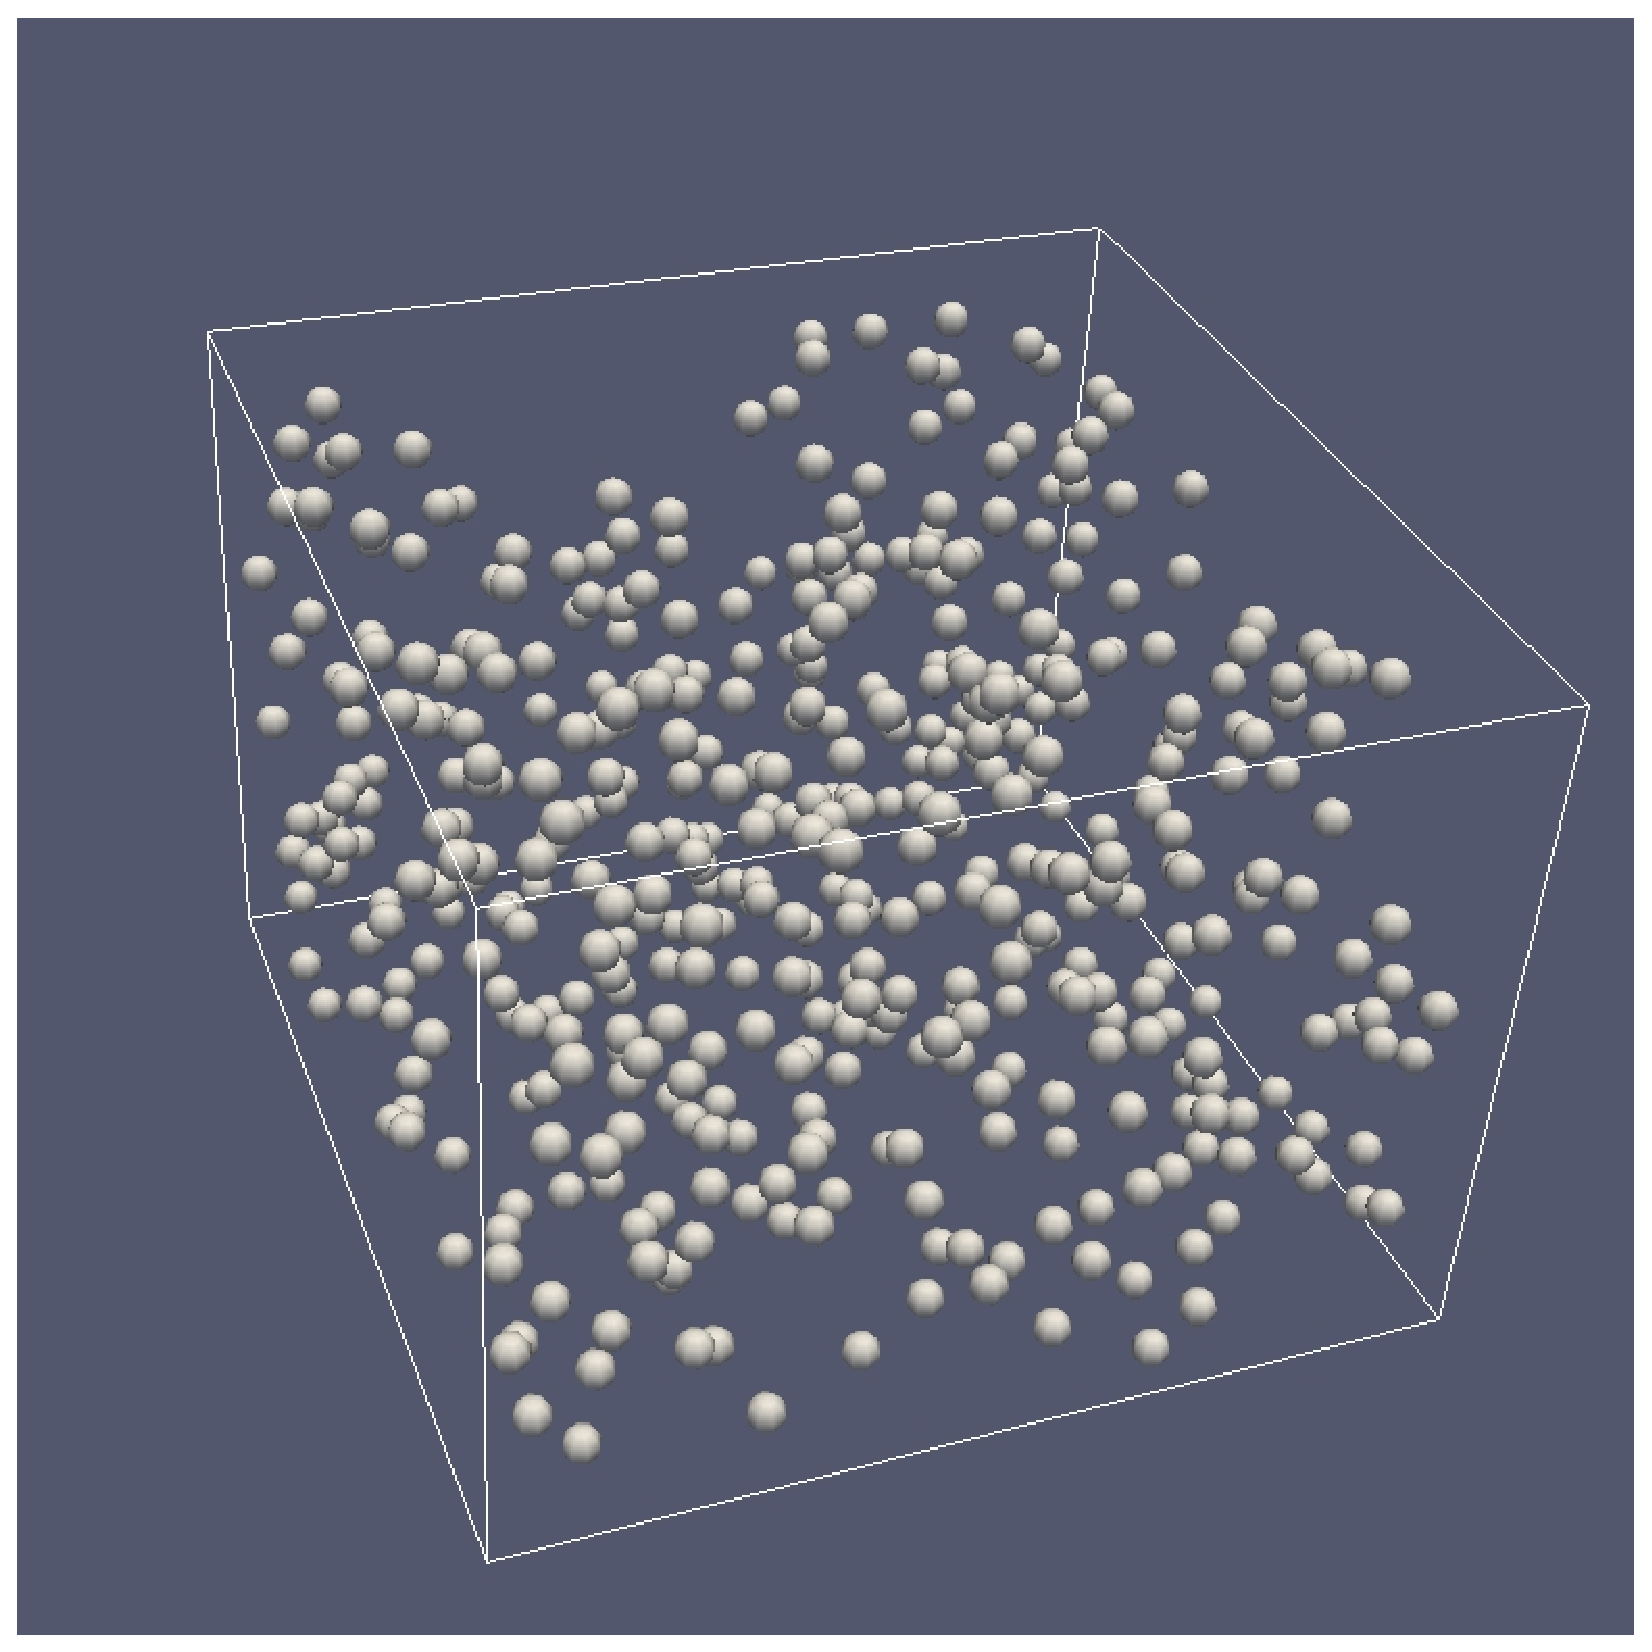
\includegraphics[width=0.45\textwidth]{compare_image_tracked3D_1}}
\end{figure}

\begin{figure}
	\ContinuedFloat
	\centering
	\subfloat
		[Superimposition of \subref{fig:compare_image_tracked3D_image} and \subref{fig:compare_image_tracked3D_plot}]
		{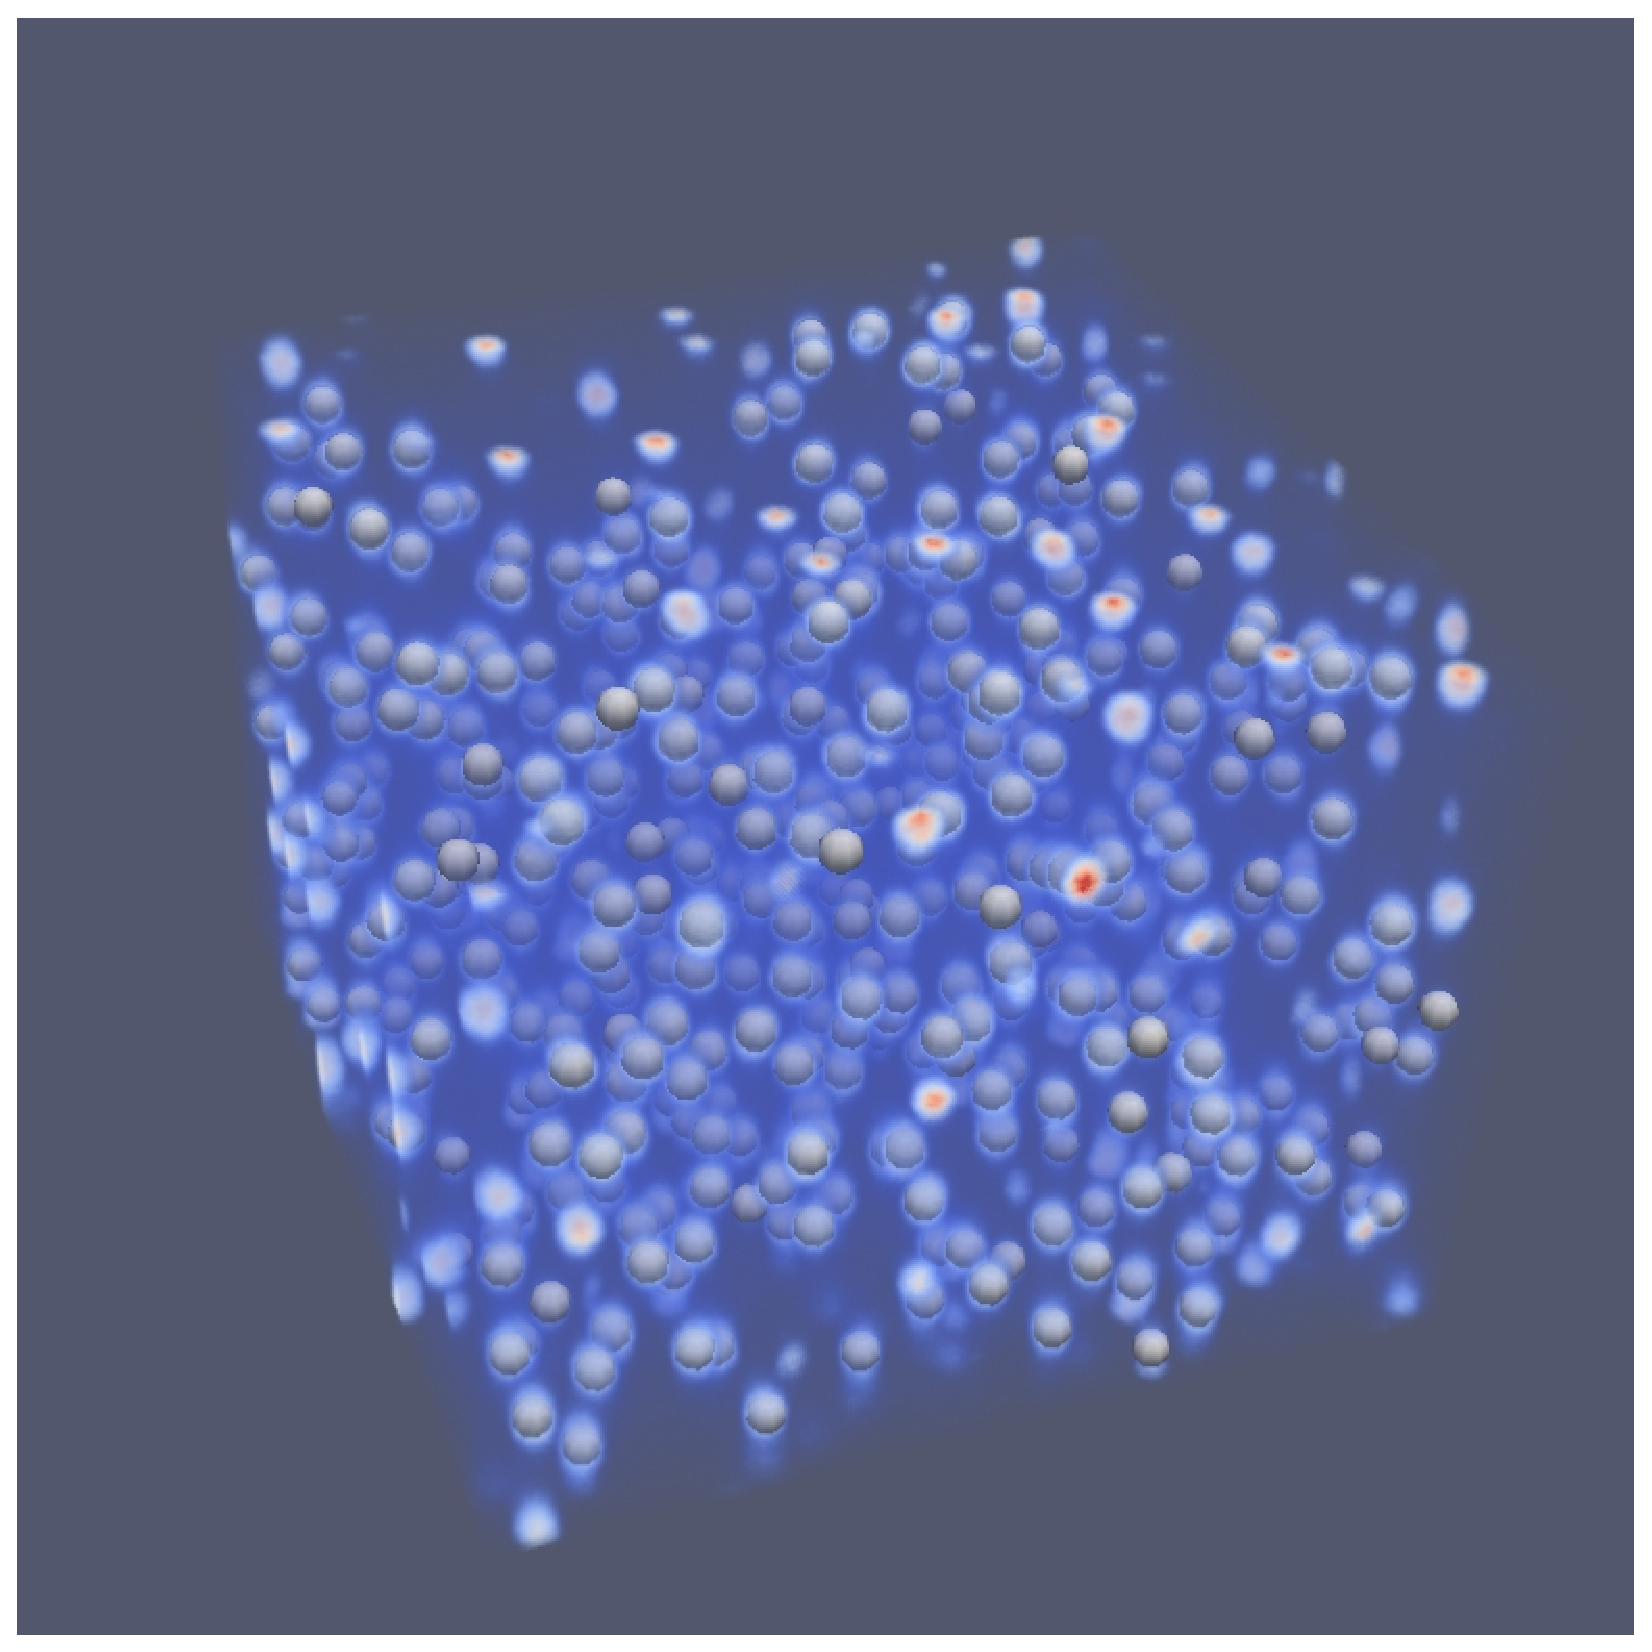
\includegraphics[width=0.8\textwidth]{compare_image_tracked3D_2}}
	\caption{Comparing the original images with the result of our tracking code in a dilute sample (for clarity). The only visible discrepancies are the absence of the particles on the boundary (discarded on purpose) and the size of the smaller particles.}
	\label{fig:compare_image_tracked3D}
\end{figure}

\subsection{Only large particles}

As we have seen in \SectionRef{sec:size_poly}, the colloids we use in experiments can have a non-negligible size polydispersity. A size distribution skewed toward small sizes is very common due to secondary nucleation during the synthesis of \ac{PMMA} particles. If the total number of particles is important to estimate the volume fraction, one can argue that some properties of the system are better caught if the tail of small particles is removed. For instance, structural properties are difficult to extract if the small particles are considered equal to the larger ones, as illustrated by \FigureRef{fig:rdf_tracking}.

\begin{figure}
	\centering
	% GNUPLOT: LaTeX picture with Postscript
\begingroup
  \makeatletter
  \providecommand\color[2][]{%
    \GenericError{(gnuplot) \space\space\space\@spaces}{%
      Package color not loaded in conjunction with
      terminal option `colourtext'%
    }{See the gnuplot documentation for explanation.%
    }{Either use 'blacktext' in gnuplot or load the package
      color.sty in LaTeX.}%
    \renewcommand\color[2][]{}%
  }%
  \providecommand\includegraphics[2][]{%
    \GenericError{(gnuplot) \space\space\space\@spaces}{%
      Package graphicx or graphics not loaded%
    }{See the gnuplot documentation for explanation.%
    }{The gnuplot epslatex terminal needs graphicx.sty or graphics.sty.}%
    \renewcommand\includegraphics[2][]{}%
  }%
  \providecommand\rotatebox[2]{#2}%
  \@ifundefined{ifGPcolor}{%
    \newif\ifGPcolor
    \GPcolortrue
  }{}%
  \@ifundefined{ifGPblacktext}{%
    \newif\ifGPblacktext
    \GPblacktexttrue
  }{}%
  % define a \g@addto@macro without @ in the name:
  \let\gplgaddtomacro\g@addto@macro
  % define empty templates for all commands taking text:
  \gdef\gplbacktext{}%
  \gdef\gplfronttext{}%
  \makeatother
  \ifGPblacktext
    % no textcolor at all
    \def\colorrgb#1{}%
    \def\colorgray#1{}%
  \else
    % gray or color?
    \ifGPcolor
      \def\colorrgb#1{\color[rgb]{#1}}%
      \def\colorgray#1{\color[gray]{#1}}%
      \expandafter\def\csname LTw\endcsname{\color{white}}%
      \expandafter\def\csname LTb\endcsname{\color{black}}%
      \expandafter\def\csname LTa\endcsname{\color{black}}%
      \expandafter\def\csname LT0\endcsname{\color[rgb]{1,0,0}}%
      \expandafter\def\csname LT1\endcsname{\color[rgb]{0,1,0}}%
      \expandafter\def\csname LT2\endcsname{\color[rgb]{0,0,1}}%
      \expandafter\def\csname LT3\endcsname{\color[rgb]{1,0,1}}%
      \expandafter\def\csname LT4\endcsname{\color[rgb]{0,1,1}}%
      \expandafter\def\csname LT5\endcsname{\color[rgb]{1,1,0}}%
      \expandafter\def\csname LT6\endcsname{\color[rgb]{0,0,0}}%
      \expandafter\def\csname LT7\endcsname{\color[rgb]{1,0.3,0}}%
      \expandafter\def\csname LT8\endcsname{\color[rgb]{0.5,0.5,0.5}}%
    \else
      % gray
      \def\colorrgb#1{\color{black}}%
      \def\colorgray#1{\color[gray]{#1}}%
      \expandafter\def\csname LTw\endcsname{\color{white}}%
      \expandafter\def\csname LTb\endcsname{\color{black}}%
      \expandafter\def\csname LTa\endcsname{\color{black}}%
      \expandafter\def\csname LT0\endcsname{\color{black}}%
      \expandafter\def\csname LT1\endcsname{\color{black}}%
      \expandafter\def\csname LT2\endcsname{\color{black}}%
      \expandafter\def\csname LT3\endcsname{\color{black}}%
      \expandafter\def\csname LT4\endcsname{\color{black}}%
      \expandafter\def\csname LT5\endcsname{\color{black}}%
      \expandafter\def\csname LT6\endcsname{\color{black}}%
      \expandafter\def\csname LT7\endcsname{\color{black}}%
      \expandafter\def\csname LT8\endcsname{\color{black}}%
    \fi
  \fi
  \setlength{\unitlength}{0.0500bp}%
  \begin{picture}(7200.00,5040.00)%
    \gplgaddtomacro\gplbacktext{%
      \csname LTb\endcsname%
      \put(1056,704){\makebox(0,0)[r]{\strut{}$0.0$}}%
      \put(1056,1286){\makebox(0,0)[r]{\strut{}$0.5$}}%
      \put(1056,1867){\makebox(0,0)[r]{\strut{}$1.0$}}%
      \put(1056,2449){\makebox(0,0)[r]{\strut{}$1.5$}}%
      \put(1056,3031){\makebox(0,0)[r]{\strut{}$2.0$}}%
      \put(1056,3613){\makebox(0,0)[r]{\strut{}$2.5$}}%
      \put(1056,4194){\makebox(0,0)[r]{\strut{}$3.0$}}%
      \put(1056,4776){\makebox(0,0)[r]{\strut{}$3.5$}}%
      \put(1188,484){\makebox(0,0){\strut{}$0$}}%
      \put(2117,484){\makebox(0,0){\strut{}$0.5$}}%
      \put(3045,484){\makebox(0,0){\strut{}$1$}}%
      \put(3974,484){\makebox(0,0){\strut{}$1.5$}}%
      \put(4903,484){\makebox(0,0){\strut{}$2$}}%
      \put(5831,484){\makebox(0,0){\strut{}$2.5$}}%
      \put(6760,484){\makebox(0,0){\strut{}$3$}}%
      \put(418,2740){\rotatebox{90}{\makebox(0,0){\strut{}$g(r)$}}}%
      \put(6979,2740){\rotatebox{90}{\makebox(0,0){\strut{}}}}%
      \put(3974,154){\makebox(0,0){\strut{}$r/\sigma$}}%
      \put(3974,4666){\makebox(0,0){\strut{}}}%
      \put(3974,4665){\makebox(0,0){\strut{}}}%
      \put(264,110){\makebox(0,0)[l]{\strut{}}}%
    }%
    \gplgaddtomacro\gplfronttext{%
      \csname LTb\endcsname%
      \put(5773,1262){\makebox(0,0)[r]{\strut{}All particles}}%
      \csname LTb\endcsname%
      \put(5773,932){\makebox(0,0)[r]{\strut{}Only the most common sizes}}%
    }%
    \gplbacktext
    \put(0,0){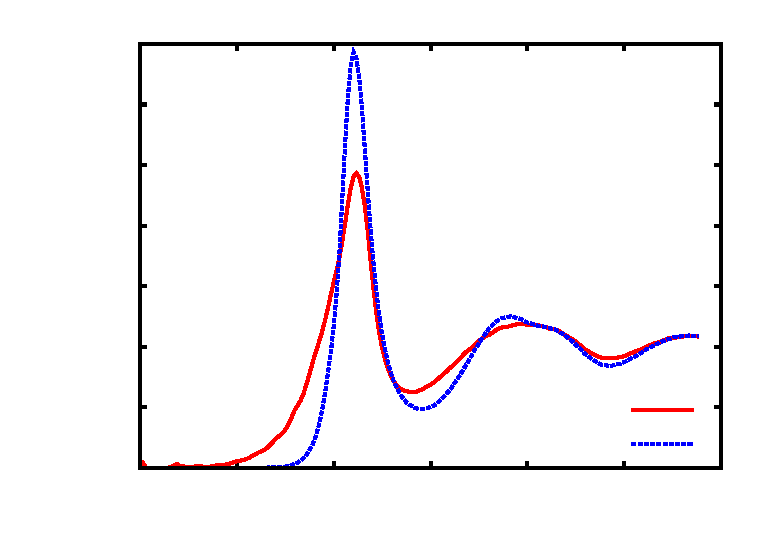
\includegraphics{./rdf_size_selection_tracking}}%
    \gplfronttext
  \end{picture}%
\endgroup

	\caption{Radial distribution function of the same sample tracked in two different ways: with $r_{min}=2.9$~pixels and $r_{max}=5.8$~pixels to catch all particles or with $r_{min}=3.4$~pixels and $r_{max}=30$~pixels to retain only the most common sizes with better precision of the coordinates.}
	\label{fig:rdf_tracking}
\end{figure}

Because our tracking algorithm cannot extract the radii with sufficient precision, we can be tempted to track our images a second time with higher values for both $r_{min}$ and $r_{max}$. Higher $r_{min}$ allows to remove the smallest particles from the filtered image, and removes also more noise leading to drastic improvement in the precision of the coordinates. Higher $r_{max}$ minimizes the filtering artefacts, increases the precision of the coordinates but disables the tracking of dim particles.

Usually we track our images two times: once to track all particles and get the number density and then a second time to get only the most common size range. The difference of number of tracked particles between the two tracking methods can be up to $20\%$ (about $10\sim15\%$ of the volume fraction). We extract the structural information from both and compare them. The small particles drastically alter the \ac{RDF}, smoothing all the peaks as shown in \FigureRef{fig:rdf_tracking}; however the \acl{BOO} (see \SectionRef{sec:boo} and \ChapterRef{ch:structure}) seems to be robust, at least for the most ordered parts of the samples. The results presented in \ChapterRef{ch:structure} corresponds to the tracking of all the sizes.

\section{Time tracking}
\label{sec:time_tracking}

As the output of the tracker, we now have $N(t)$ particle locations at each time $t$, with $N(t) \neq N(t')$ in general. Contrary to a typical simulation output, the number of particle is not constant in time, particles are coming in and out of the field of view, and the particles are truly indistinguishable, with no index to tell them apart. To analyse the dynamics of our system, we need to link the locations into trajectories.

\subsection{Proximity criterion}

The only way to link the location $r_i(t)$ to one of the locations of the next time step $\lbrace r_j(t+1) \rbrace_{j\in N(t+1)}$ is a proximity criterion. We have to suppose that during the unit time interval, any particle moved only a fraction of the typical inter-particular distance. Then, the right $r_j(t+1)$ is the one minimizing the distance $\left\| r_j(t+1) - r_i(t)\right\|$. This is a well-known optimization problem called "all nearest neighbours" that requires $O(N!)$ operations if solved by brute force. The set of possible links forms a network of $N(t)N(t+1)$ bonds.

Crocker and Grier suggested to use only the links shorter than the typical inter-particular distance. The network then reduces to a collection of disconnected sub-networks. Most of the sub-networks contain only one link and are resolved in $N \log N$ operations by most implementations. A sub-network that links $M$ particles to $M$ particles ($M \ll N$) is solved in $O(M!)$ operations at most (often fewer). Some trajectories finish and some trajectories start at each time step.

\subsection{Validity of the hypothesis}

The previous proximity criterion presuppose that any particle moved only a fraction of the typical inter-particular distance $L$ between two consecutive images. A single Brownian particle diffuses its own radius $L$ in the time $\tau_B = \frac{L^2}{2 d D_0}$, with $D_0$ the diffusion coefficient at infinite dilution and $d$ the dimension of space. To allow time tracking of a dilute sample, one need to take a 3D picture every $dt\ll\tau$. With our samples, it means $dt\sim \unit{2}{\second}$.

In dense samples, trajectory linking is paradoxically easier because the diffusion is not free: the dynamics is activated and particles move by hops of a fraction of their diameter. The time interval between two pictures can then be much longer, depending on the volume fraction. A liquid at the limit of supercooling can be tracked with an interval of \unit{5}{\second}. At $\phi=0.55$, \unit{30}{\second} is sufficient. Deeply supercooled liquids allow trajectory linking even with intervals as long as \unit{30}{\minute}.

\subsection{Improvement by spatial query}

Rather than calculating the length of all the possible links, we used the spatial queries described in \SectionRef{sec:spatial_query} to select quickly the possible links. With this method, the reduced network is constructed in $O(N(t)\log N(t+1)$ operations and contains only $P=n N(t)$ potential links, with $1\leq n \leq 2$.

\subsection{Keep only the shortest}

We can then sort the potential links by increasing length. This is done in $O(P\log P)$ operations. By definition, the shortest potential link minimizes the proximity criterion: it is a good link. Let us note $p$ and $q$ the locations of the beginning (time $t$) and the end (time $t+1$) of this link. If there exist other potential links starting from $p$ or ending at $q$, they are longer than our link $(p, q)$, so they are not good links, so we discard them. The remaining links are still sorted by increasing length and the shortest is a good link. We continue this procedure until no potential link is left. At the end of this algorithm, we have selected the subset of potential links that minimizes the proximity criterion. All the trajectories that have not found a location at $t+1$ finish. All locations that are not linked to an existing trajectory are the starting point of a new trajectory.

The key of the efficiency of this algorithm is the time to find and discard all the links that contains $p$ or $q$. Brute force searching takes $N_{link}$ comparisons for $p$ and the same for $q$, so a total cost of $O(P \times N)$. To find them more quickly, we can index the set of potential links in both $p$ and $q$, independently. That reduces the searching cost to $O(P\log P)$ operations.

\subsection{Implementation using a bidirectional map}

Maintaining two indices on a constantly updating set of objects can be a pain for a non-professional programmer and thus terribly error prone. Thankfully, the boost libraries~\citep{boost} provides a structure called bidirectional map, inspired by \ac{RDMS}, that does exactly the work needed here. It is a set of pairs $(p,q)$, indexed by both keys. This structure enforces the uniqueness of each $p$ and each $q$. That is to say that, if one wants to insert a pair whose first element is already the first element of another pair, then the insertion is silently ignored. This is the same for the second element. Checking the uniqueness before insertion costs $O(\log G)$ with $G \leq N$ the number of good links already inserted.

With the bidirectional map, the linking algorithm becomes very simple. Once the potential links are sorted by increasing length ($O(P \log P)$), they are inserted one by one into the bidirectional map. Bad links are automatically not inserted. Each tentative insertion costs $O(\log G)$, for a total of $O(P \log G)$. New trajectories are started if needed. To sum up, the linking operation behaves at most like $O(N\log N)$.

\section{Other improvements}

\subsection{Reading Leica files}

Thanks to the open-source software community, we could find and integrate into our tracking software a piece of code~\citep{kankaanpaa2006bioimagexd} that reads \ac{LIF}, the (proprietary, undocumented) output format of our microscope. Before, the data needed to be exported as 2D TIFF images (one per $XY$ slice) and then read back into the tracking code. This step was consuming hours of disk I/O time for nothing.

\subsection{Deshaking}

When the time interval between image acquisition is set to more than \unit{1}{\minute}, some overall displacement of the sample appears between time steps. The amount of displacement can be larger than the size of the particles, breaking completely the linking hypothesis. This very annoying effect remained a mystery for weeks. We first thought it was due to flow in the sample, so we doubled-checked the glue sealing the capillary and investigated the temperature control.The seismic activity of Japan, the walking of people nearby or the air flux of the air conditioner could not be accused because our microscope is standing on a vibration isolation table and the displacement was periodic with a period of a few minutes. Finally, we discovered that this displacement was due to the automatic realignment of the microscope stage that is impossible to disable.

We had to find a way to get rid of the global drift by post-processing the data. This is actually a very active field of research in applied optics and is called "digital image stabilization" on commercial digital video cameras. In our case (two almost identical but translated images), it is rather called "image registration". This type of method was developed originally to register a set of satellite pictures into a larger map~\citep{Brown1992}. The simpler and most robust method is the phase correlation alignment method~\citep{kuglin1975phase} based on the Fourier shift theorem. 

Given two input images $g_a$ and $g_b$, we apply a window function (\latin{e.g.}, a Hamming window) on both images to reduce edge effects. Then, we calculate the discrete 2D Fourier transform of both images:
\begin{align}
\mathbf{G}_a = \mathcal{F}\{g_a\} \\
\mathbf{G}_b = \mathcal{F}\{g_b\}
\end{align}
and calculate the cross-power spectrum $R$ and its inverse Fourier transform, the the normalized cross-correlation $r$:
\begin{align}
    R = \frac{ \mathbf{G}_a \mathbf{G}_b^*}{\left\|\mathbf{G}_a \mathbf{G}_b^*\right\|} \\
    r = \mathcal{F}^{-1}\{R\} 
\end{align}

If the two pictures are actually not too different one from the other, and that the images present no periodic patterns, then the result is a noisy dark background with a single bright peak. The position of this peak gives the translation between the two pictures.

Rather than actually translate the pictures, the particle localization is done on the original image. However, before linking trajectories the coordinates are translated to correct the overall displacement (see \FigureRef{fig:tracking_process}).

Recently~\citep{Besseling2009}, this method was used to track non-uniform flows of particles. The phase correlation alignment method was applied on every slice to reconstruct a complex shear profile. Because our global displacement was uniform in the $XY$ plane, we apply this method in 2D only on the the middle slice of the 3D stack.
%\newpage
% Create the bibliography right after the text
%\bibliographystyle{ieeetr}
%\bibliography{mathieu}